\documentclass{beamer}

\usepackage{beamerthemeparktex}
\graphicspath{ {./images/} }

\setbeamerfont{title}{series=\bfseries,parent=structure}

\title{\textcolor{nord10}{Parkview}}
\subtitle{\textcolor{nord9}{Performance Dashboard for continuous Benchmarking of HPC Libraries}}
\author{Chingun Ariunbat, Jamil Bagga, Walter Alexander B\"ottcher, Darius Schefer, Maximilian Schik}

\setcounter{tocdepth}{1}

\begin{document}

\maketitle

\begin{frame}{Table of Contents}
  \tableofcontents
\end{frame}

\section{General Overview}
\begin{frame}
  \begin{center}
    \Huge{General Overview}
  \end{center}
\end{frame}

\subsection{Continuous Benchmarking}
\begin{frame}{Continuous Benchmarking}
  \begin{itemize}
      \item Problem: Keeping track of software performance
      \item Solution: Run benchmarks on every (major) change, similar to continuous testing
      \item How to inspect the results?
  \end{itemize}
\end{frame}

\subsection{Parkview To The Rescue}
\begin{frame}{Parvkiew To The Rescue}
  \begin{itemize}
      \item Goal: Create a product that helps the user to:
        \begin{itemize}
          \item Organize Benchmark Results
          \item Create customizable plots
          \item Compare the performance over different commits
        \end{itemize}
      \item Our solution to the problem: Parkview
  \end{itemize}
\end{frame}

\section{Demo}
\begin{frame}
  \begin{center}
    \Huge{Demo Time}
  \end{center}
\end{frame}

\section{Code Time}
\begin{frame}
  \begin{center}
    \Huge{Code Time}
  \end{center}
\end{frame}

\subsection{Statistics}
\begin{frame}{Statistics}
  \begin{itemize}
      \item 2986 lines of backend code
      \item 3433 lines of frontend code
      \item 73\% percent backend line coverage
      \item 41\% percent frontend line coverage
      \item 803 commits, 33 issues resolved, 58 pull requests merged
  \end{itemize}
\end{frame}

\subsection{Quick'n Dirty Code Review}
\begin{frame}{Quick'n'Dirty Code Review}
  \begin{center}
    \large{SYSTEM MODEL IMAGE}
  \end{center}
\end{frame}

\subsection{Extensibility}
\begin{frame}{Extensibility}
  \begin{itemize}
    \item For new plot types only changes to the backend are needed
    \item Frontend renders all available options and just passes them back to the backend
    \item Adding a new plot is done by adding a single new class
  \end{itemize}
\end{frame}

\section{Continuous Integration}
\subsection{Pipeline}
\begin{frame}{Pipeline}
  \begin{columns}
    \column{0.5\textwidth}
    \begin{itemize}
      \item Containers are built in the \textit{build-*} phases and are reused in the \textit{integration} and \textit{push-*-container} phases
      \item The \textit{build-*-container} phases push the built containers to DockerHub (only on changes to the \texttt{develop} or \texttt{release} branch)
      \item The \textit{deploy} phase deploys the software to a remote server (only on changes to the \texttt{develop} branch)
    \end{itemize}
    \column{0.5\textwidth}
    \begin{figure}
      \begin{center}
        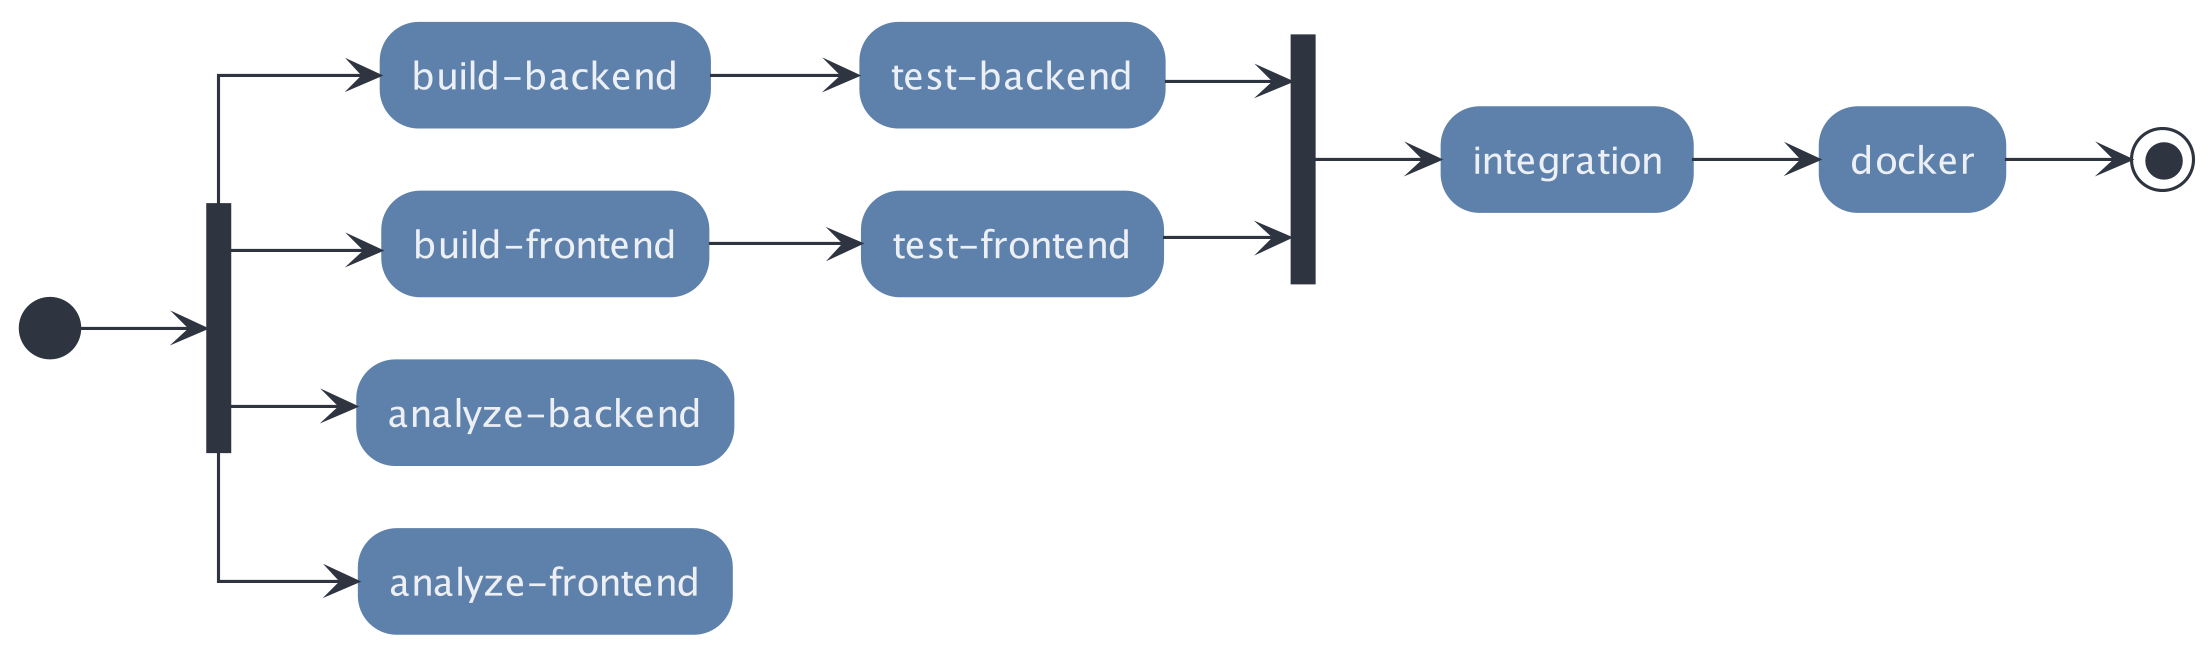
\includegraphics[scale=0.09]{ci_activity}
        \caption{Activity diagram of CI pipeline}
      \end{center}
    \end{figure}
  \end{columns}
\end{frame}

\subsection{Containerization}
\begin{frame}{Containerization}
  \begin{itemize}
    \item Made development and especially deployment much easier
    \item People working on the frontend didn't have to bother with compiling the backend or setting up a database and the other way around
    \item Made continuous deployment a one line shell script: \texttt{docker-compose down \&\& docker-compose pull \&\& docker-compose up -d}
  \end{itemize}
\end{frame}

\section{Our Experiences}

\begin{frame}
  \begin{center}
    \Huge{Our Experiences}
  \end{center}
\end{frame}

\begin{frame}{Max}
  \begin{itemize}
    \item I learned a lot about "meta development"
    \item I learned how to \textbf{NOT} write software (waterfall model)
    \item Putting everything behind an interface is suprisingly efficent
    \item Leveraging GitHub for cooperation
    \item After redoing something $\sim$ 20 times it starts looking decent
    \item Tests make me less paranoid
  \end{itemize}
\end{frame}

\begin{frame}{Darius}
  \begin{itemize}
    \item I learned a lot about Angular
    \item And responsive web development in general
    \item I understand git a lot better
    \item I learned a lot more about Latex
    \item My Latex workflow also is a lot more efficient now
  \end{itemize}
\end{frame}

\begin{frame}{Chingun}
    \begin{itemize}
        \item What you learned
    \end{itemize}
\end{frame}

\begin{frame}{Joe}
    \begin{itemize}
        \item What you learned
    \end{itemize}
\end{frame}

\begin{frame}
  \begin{center}
    \Huge{I hope you enjoyed listening to this presentation as much as we enjoyed writing it!}
  \end{center}
\end{frame}

\end{document}
